% !TEX TS-program = pdflatex
% !TEX encoding = UTF-8 Unicode

% This is a simple template for a LaTeX document using the "article" class.
% See "book", "report", "letter" for other types of document.

\documentclass[11pt]{article} % use larger type; default would be 10pt

\usepackage[utf8]{inputenc} % set input encoding (not needed with XeLaTeX)

%%% Examples of Article customizations
% These packages are optional, depending whether you want the features they provide.
% See the LaTeX Companion or other references for full information.

%%% PAGE DIMENSIONS
\usepackage{geometry} % to change the page dimensions
\geometry{a4paper} % or letterpaper (US) or a5paper or....
% \geometry{margin=2in} % for example, change the margins to 2 inches all round
% \geometry{landscape} % set up the page for landscape
%   read geometry.pdf for detailed page layout information

\usepackage{graphicx} % support the \includegraphics command and options

% \usepackage[parfill]{parskip} % Activate to begin paragraphs with an empty line rather than an indent

%%% PACKAGES
\usepackage{booktabs} % for much better looking tables
\usepackage{array} % for better arrays (eg matrices) in maths
\usepackage{paralist} % very flexible & customisable lists (eg. enumerate/itemize, etc.)
\usepackage{verbatim} % adds environment for commenting out blocks of text & for better verbatim
\usepackage{subfig} % make it possible to include more than one captioned figure/table in a single float
% These packages are all incorporated in the memoir class to one degree or another...

%%% HEADERS & FOOTERS
\usepackage{fancyhdr} % This should be set AFTER setting up the page geometry
\pagestyle{fancy} % options: empty , plain , fancy
\renewcommand{\headrulewidth}{0pt} % customise the layout...
\lhead{}\chead{}\rhead{}
\lfoot{}\cfoot{\thepage}\rfoot{}

%%% SECTION TITLE APPEARANCE
\usepackage{sectsty}
\allsectionsfont{\sffamily\mdseries\upshape} % (See the fntguide.pdf for font help)
% (This matches ConTeXt defaults)

%%% ToC (table of contents) APPEARANCE
\usepackage[nottoc,notlof,notlot]{tocbibind} % Put the bibliography in the ToC
\usepackage[titles,subfigure]{tocloft} % Alter the style of the Table of Contents
\renewcommand{\cftsecfont}{\rmfamily\mdseries\upshape}
\renewcommand{\cftsecpagefont}{\rmfamily\mdseries\upshape} % No bold!

\usepackage{setspace}
\onehalfspacing

\usepackage{float}

%Reference%
\usepackage{apacite}

%Table%
\usepackage{tabularx}
\usepackage{booktabs}
\usepackage{makecell} 
\usepackage{longtable}

%Image%
\usepackage{graphicx}
\usepackage{caption} 
\graphicspath{ {./images/} }

%Code%
\usepackage{listings}
\usepackage{xcolor}
\definecolor{codegreen}{rgb}{0,0.6,0}
\definecolor{codegray}{rgb}{0.5,0.5,0.5}
\definecolor{codepurple}{rgb}{0.58,0,0.82}
\definecolor{backcolour}{rgb}{0.95,0.95,0.92}

\lstset{
	numbers=left,
	numberstyle=\tiny,
	xleftmargin=2em,
	basicstyle=\small,
	commentstyle=\color{codegreen},
	keywordstyle=\color{magenta},
	columns=fullflexible,
	breaklines=true
	showspaces=false,                
	showstringspaces=false,
	showtabs=false,                  
	tabsize=2
}


%%% END Article customizations

%%% The "real" document content comes below...

\title{3st Assignment COMPX523-25A}
\author{}
%\date{} % Activate to display a given date or no date (if empty),
% otherwise the current date is printed 

\begin{document}
\maketitle

%Contents%
\pagenumbering{roman}
\tableofcontents
\newpage
\pagenumbering{arabic}
	
\section{Abstract}

\section{Introduction}

Increasing urbanisation around the world has resulted in an increasing demand for public transport services, particularly in developing countries. However, financial and infrastructure constraints have made it difficult for governments to match this growing demand \cite{motta2013crisis}. The public transport crowding that has resulted from this causes increased stress, increased unreliability of public transport services, and reduced productivity for passengers \cite{tirachini2013crowding}.

Intelligent Public Transport Systems (IPTS) is a nascent field that attempts to address issues with public transport using machine learning (ML) \cite{zear2016intelligent}. Accurate prediction of public transport volumes is one way that ML can be leveraged to improve public transport and reduce crowding. If passenger volumes are known ahead of time, it may be possible for public transport agencies to optimise the availability of buses and trains in order to match demand and thus reduce crowding. Passengers can also directly benefit from foreknowledge of the demand at a given station or bus route, as they can plan their travel to avoid crowding \cite{di2024machine}.

The data stream mining paradigm is designed for large quantities of data which arrive continuously, in a setting where memory and computational power might be constrained \cite{bifet2023machine}. Public transport data fits this paradigm, thus the field of data stream mining provides us with a set of ML algorithms that are appropriate for deployment in this context.

The setting of this study is Salvador, the fifth largest city in Brazil. Compared to other metropolitan areas in Brazil, there is a higher reliance on public transport in Salvador due to a broadly lower socioeconomic status. The majority of public transport in Salvador is by bus, although some passengers take the Salvador Metro \cite{harrison2016brics}. The Salvador Urban Network Transportation (SUNT) dataset contains high granularity information about passenger volumes at bus stops and stations across Salvador, between March and May 2024 \cite{SUNT2025}.

The aim of this study is to investigate data stream ML models by which the load of passengers on buses in Salvador can be estimated. Such models, if deployed, could be used by agencies or passengers to accurately estimate the moment-by-moment demand at each of these bus stops. These models could also be inspected using explainable AI techniques to gain insights into what factors influence public transport demand in Salvador.

\section{Background}
This study analyzes time series data provided by public transport datasets from 10 stations in a large Brazilian city. The datasets include boarding\_03-05\_2024.csv, landing\_03-05\_2024.csv, and loader\_03-05\_2024.csv, which contain accumulated data at 5-minute and 30-minute intervals. These files respectively represent boardings, landings, and loader (bus occupancy), as shown in the table~\ref{tab:data_source}. The time range spans from 05:00:00 on 1 March, 2024, to 00:55:00 on 31 May, 2024.

\begin{table}[H]
	\centering
	\caption{Data Source}
	\label{tab:data_source}
	\resizebox{\textwidth}{!}{
	\begin{tabular}{|l|l|}
		\hline
		\textbf{Data} & \textbf{Source} \\ \hline
		Boarding & \makecell[l]{Data mining techniques from Automatic Vehicle Location (AVL), \\Automatic Fare Collection (AFC), and \\General Transit Feed Specification (GTFS) systems} \\ 
		Alighting & Trip chaining method \\
		Bus occupancy & Ratio of boardings and alightings per vehicle \\ \hline
	\end{tabular}
	}
\end{table}

This study uses the bus occupancy of 5-minute time series data (Figure~\ref{fig:loader}) and finds that some bus stops experience heavy passenger flows during certain periods, while others often remain sparsely used.

\begin{figure}[H]
	\centering
	\caption{Bus Occupancy}
	\label{fig:loader}
	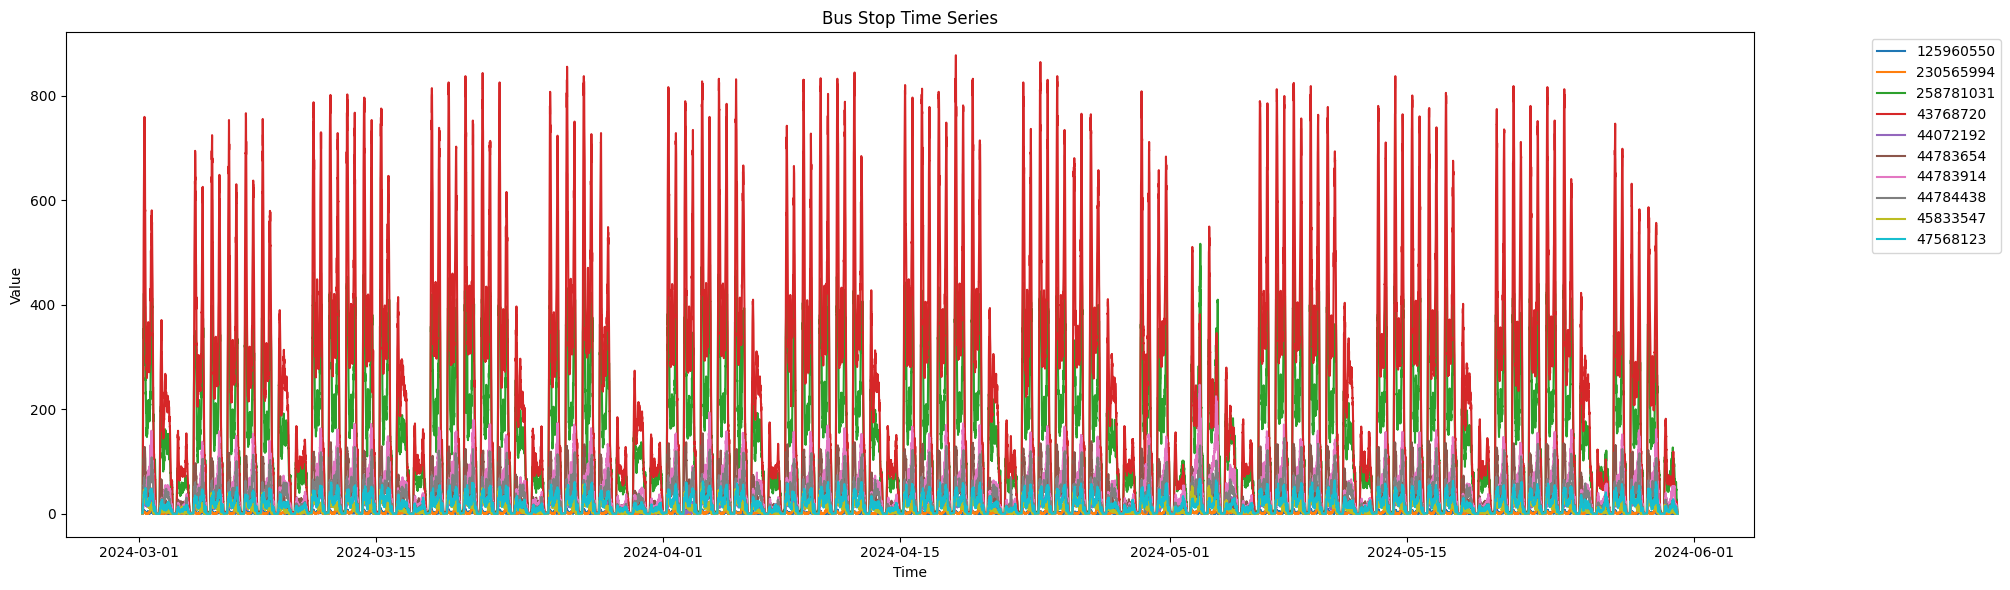
\includegraphics[scale=0.3]{loader}
\end{figure}

The reasons for the large passenger flows at certain stations shown in Table~\ref{tab:bus_stops}:
\begin{table}[H]
	\centering
	\caption{Bus Stop}
	\label{tab:bus_stops}
	\resizebox{\textwidth}{!}{
		\begin{tabular}{|l|l|l|}
			\hline
			\textbf{Stop ID} & \textbf{Location} & \textbf{Observations} \\
			\hline
			44783654 & \makecell[l]{In front of the \\Federal University of Bahia (UFBA)} & High volume of students and university staff \\
			43768720 & Lapa Station & One of the city's main public transport terminals \\
			230565994 & Itapuã Lighthouse Beach & \makecell[l]{Passenger flow varies throughout the day; \\higher on weekends and holidays} \\
			125960550 & Arena Fonte Nova surroundings & Demand influenced by sports and cultural events \\
			45833547 & Near Manoel Barradas Stadium & Sharp increases in demand during game days \\
			44784438 & Near the Ferry Boat terminal & Primarily serves intercity and cross-bay travelers \\
			47568123 & Near a major shopping mall & High commercial traffic throughout the day \\
			44072192 & Close to Castro Alves Theater & \makecell[l]{Passenger flow increases \\during performance and event hours} \\
			258781031 & Salvador Bus Station & Central hub for urban and intercity bus routes \\
			44783914 & Lacerda Elevator tourist area & Located in a busy commercial and tourist district \\
			\bottomrule
		\end{tabular}
	}
\end{table}

The surge in passenger volume is caused by some objective patterns.
For example, during an annual event held near a specific stop, such as a sports competition or cultural celebration, a large number of people tend to take buses to that location. As a result, the bus routes near the stop become unusually busy and may even lead to traffic congestion. Passengers who are unaware of the situation might further worsen the congestion.

\section{Proposal}
To address the problem of congestion caused by high passenger flow,
we propose a station recommendation system,
which analyzes the busyness of transit stops and provides real-time suggestions for alternative stations. In this way, passengers can avoid overcrowded stops,
thereby reducing congestion and improving travel efficiency. 

By integrating the CapyMOA online learning algorithm,
the system is able to adapt dynamically to changes in passenger flow and offer station recommendations.

\subsection{System Design}
The station recommendation system consists of two core tasks: First, identifying busy stations by using 5-minute aggregated data to detect stations with high passenger flow in real time. Second, recommending alternative stations that are nearby and have lower traffic, in order to balance the transportation load.

\subsection{System Achitecture}
Passengers can use the station recommendation system to check whether a stop is crowded. If the queried station is busy, the system predicts the station with the lowest passenger flow at the current time and calculates the nearest stop to recommend. This helps passengers avoid congested stops, as shown in the Figure~\ref{fig:achitecture}.

\begin{figure}[H]
	\centering
	\caption{Achitecture}
	\label{fig:achitecture}
	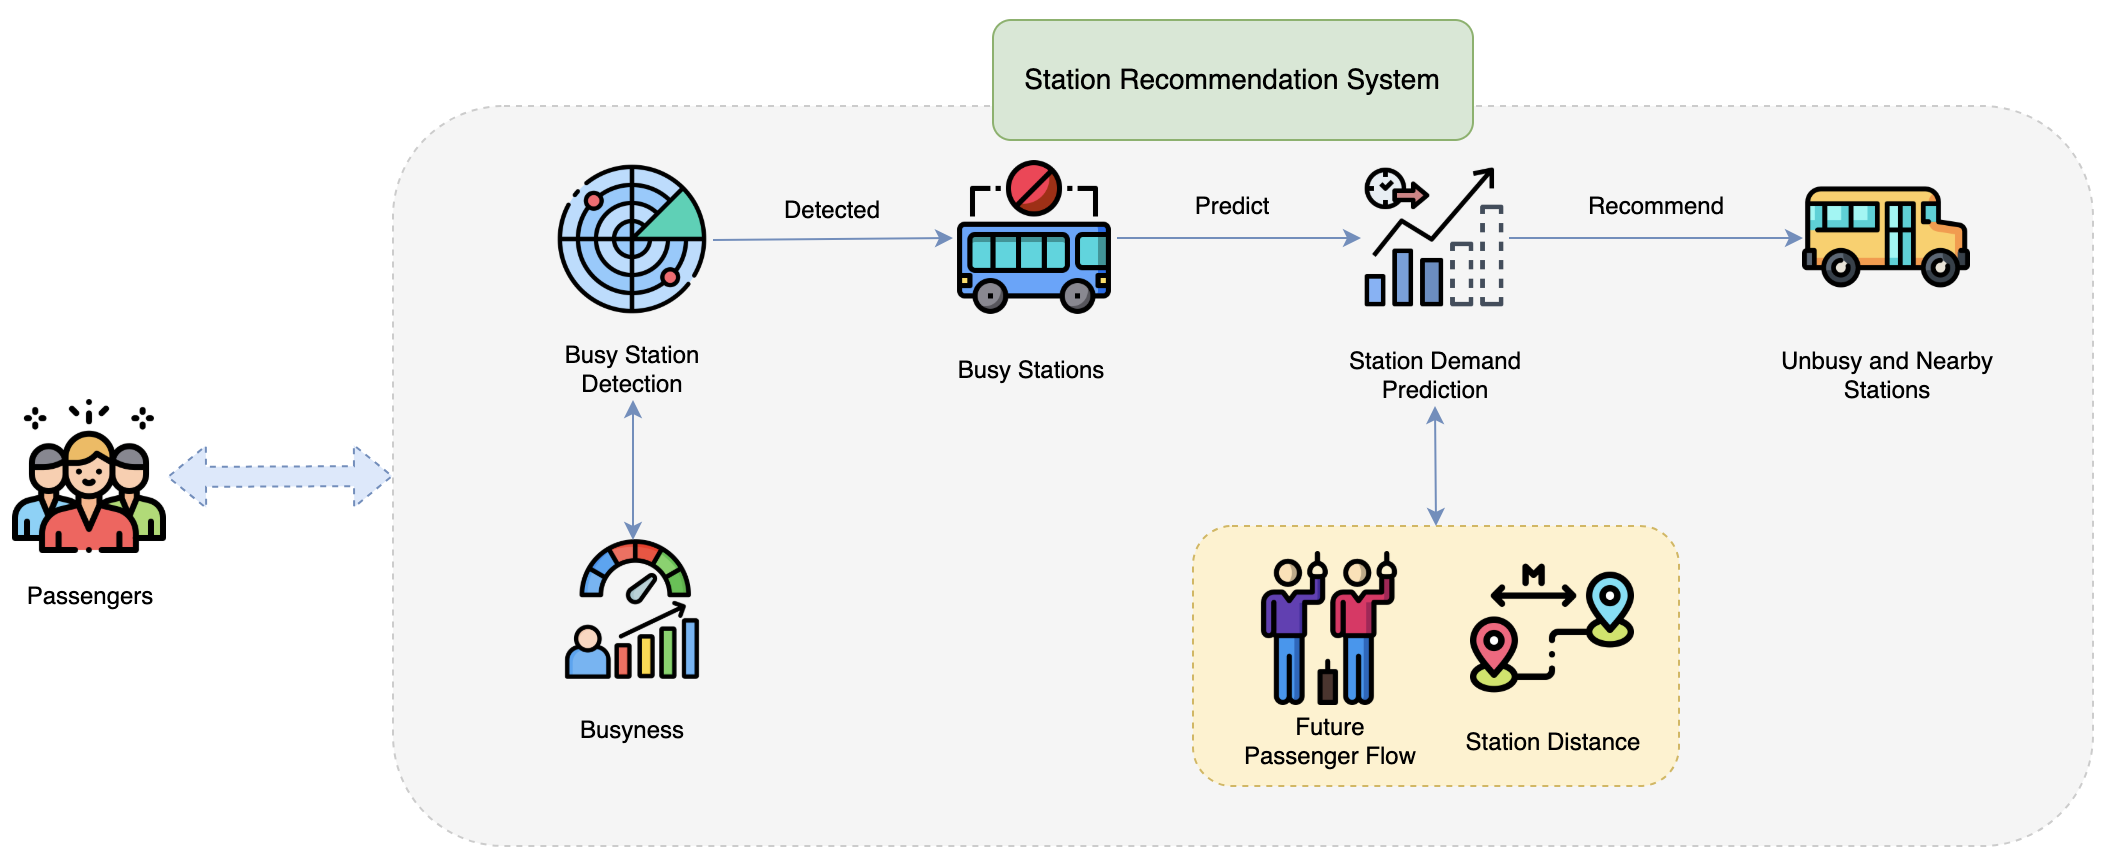
\includegraphics[scale=0.4]{architecture}
\end{figure}

\section{Experiments}
\subsection{Data Preparation}
This study analyzes both 5-minute and 30-minute aggregated data. The 5-minute data is more suitable for monitoring real-time passenger flow. Based on the two main tasks of the system, we propose building two separate models: the Busy Station Detection (BSD) Model and the Station Demand Prediction (SDP) Model.

\subsubsection{Features and Label Design}
The BSD task is defined as a classification problem. The goal is to generate a set of features for each station at a specific time, which will be used for model training. The designed features include:

\begin{enumerate}
\item Boarding, Landing, and Loader: These are the number of boardings, landings, and onboard passengers at the current station and time. If the data is missing, the value is set to 0.
\item Hour, Day of Week, and Is Weekend: Time-related features, including the hour of the day, day of the week, and whether it is a weekend.
\item  Nearby Flow: The total number of onboard passengers at the three nearest stations at the current time.
\end{enumerate}

The label is binary classification, indicating whether a station is busy (0 means not busy, 1 means busy). According to local regulations and vehicle types in Salvador, Brazil, the maximum passenger capacity of public buses depends on the model:

\begin{enumerate}
\item Standard single-unit buses: about 70 to 90 people (including seated and standing passengers).
\item Articulated buses (articulado): about 120 to 150 people (longer buses with more capacity).
\end{enumerate}

Therefore, we set an absolute minimum passenger threshold of 100 people to exclude stations with very low traffic and reduce noise.

We use the Z-score standardization method. Assuming the data follows a normal distribution, a Z-score greater than 1.5 corresponds to approximately the 93.3rd percentile, meaning the station’s passenger flow is higher than 93.3\% of all stations.

For each station's passenger flow $x_i $ (total passengers), the Z-score is calculated as:

\begin{equation}
	z_i = \frac{x_i - \mu}{\sigma + \epsilon}
	\label{eq:zscore}
\end{equation}

Where:

\begin{enumerate}
\item $\mu$: Mean passenger flow of all stations;
\item $\sigma$: Standard deviation of all station passenger flows;
\item $\epsilon$: A very small value (e.g., $1 \times 10^{-6}$) to avoid division by zero.
\end{enumerate}

Based on this analysis, we define the set of busy stations $S$ as those that meet both of the following conditions:

\begin{equation}
	S = \{ i \mid z_i > 1.5 \land x_i > 100 \}
\end{equation}

\begin{enumerate}
\item $z_i > 1.5$: The passenger flow is significantly higher than the average (Z-score threshold);
\item $x_i > 100$: The absolute number of passengers exceeds the minimum threshold
\end{enumerate}

The SDP Model is a regression learner. It uses the same features as the BSD Model, but the label is the passenger flow in the next time period, which is of type 'numeric'. For example, given a time period (timestamps), the target is to attain the passenger flow in the next time period, that is:

\begin{equation}
	target\_timestamp = timestamp + 1
\end{equation}

\subsubsection{Calculate Distance}
To recommend alternative stations when one becomes busy, we need to find replacement stations within 1000 meters. To do this, we calculate the distance between two stations. Although the Haversine formula is more accurate for geographic distance, we simplify the calculation using the Euclidean distance formula.

Let:
\begin{enumerate}
\item  $lat_1, lon_1$: Latitude and longitude of station 1;
\item  $lat_2, lon_2$: Latitude and longitude of station 2;
\end{enumerate}

The simplified Euclidean distance $d$ (in degrees) is:
\begin{equation}
	d = \sqrt{( lat_1 - lat_2 )^2 + ( lon_1 - lon_2 )^2}
\end{equation}

Since the result is in degrees, we need to convert it into meters. Near the equator:

\begin{equation}
	1^\circ \approx 111{,}000 meters 
\end{equation}

So the final distance in meters:
 \begin{equation}
 	D = d \times 111{,}000
 \end{equation}
 
\subsubsection{Recommend Alternative Stations}
To predict and recommend nearby stations with lower future passenger flow, the system follows these steps:

\begin{enumerate}
	\item Calculate the distance between the current busy station and all other stations, and sort them from nearest to farthest.
	\item Select the top five nearest stations, and for each station:
	
		\begin{enumerate}
			\item Extract its features.
			\item Predict the station's future passenger flow using the SDP Model, and record the result.
			\item Compute the distance between the busy station and the candidate station.
		\end{enumerate}
		
	\item Generate a set of recommended stations, where each station includes the following information:
	
	\begin{enumerate}
		\item Station name
		\item Predicted passenger flow
		\item Distance from the busy stationdistance
		\item A final score, calculated as:
		\begin{equation}
			score = \frac{predicted\_flow + 1}{distance}
		\end{equation}
		The lower the score, the better the recommendation. A lower score indicates closer distance and lower predicted flow.
	\end{enumerate}
	
	\item Finally, sort all candidate stations in ascending order by their score, and return the top two recommended stations.
\end{enumerate}

\subsection{Results}
The BSD Model uses Hoeffding Adaptive Tree (HAT). HAT is an adaptive incremental decision tree algorithm designed for data stream environments. It is especially suitable for non-static data that changes over time. When classifying station status (busy or not busy) in real time, HAT can quickly adapt to sudden changes in passenger flow patterns.

\begin{figure}[H]
	\centering
	\caption{Accuracy of Busy Station Detection Model}
	\label{fig:hat_plot}
	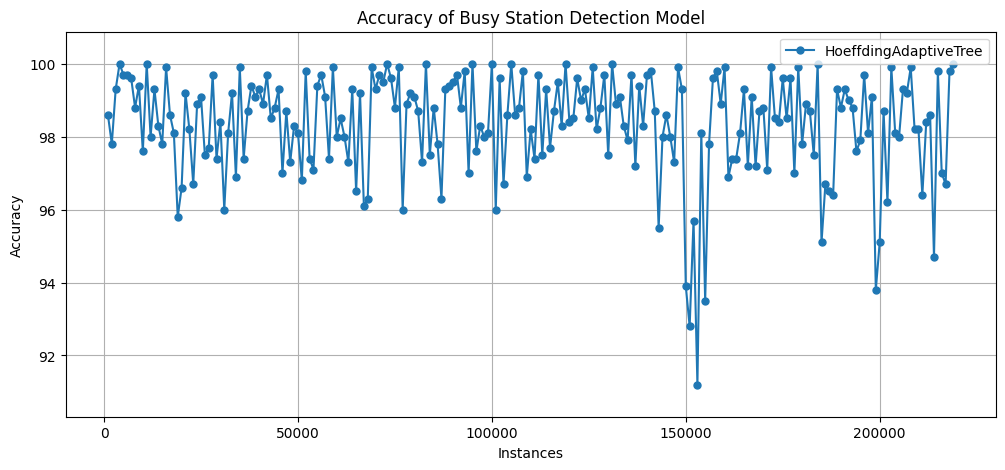
\includegraphics[scale=0.55]{hat_plot}
\end{figure}

The accuracy in most windows ranges between 96\% and 100\% shown in Figure~\ref{fig:hat_plot}, with only a few windows experiencing brief drops, but overall fluctuations are minor. There are a few dips, such as around the 150,000 and 180,000 sample marks, where accuracy drops significantly, reaching as low as 91\%. These declines may correspond to concept drift in the data distribution, but the model quickly recovers afterward, indicating that HAT has strong adaptability. 

The SDP Model uses FIMT-DD (Fast Incremental Model Tree with Drift Detection). FIMT-DD is an incremental regression tree algorithm for predicting continuous numeric values. When predicting future passenger demand (e.g., the next 5-minute period), FIMT-DD can capture both trend changes and unexpected fluctuations effectively.

\begin{figure}[H]
	\centering
	\caption{Adjusted R2 of Station Demand Prediction Model}
	\label{fig:r2_plot}
	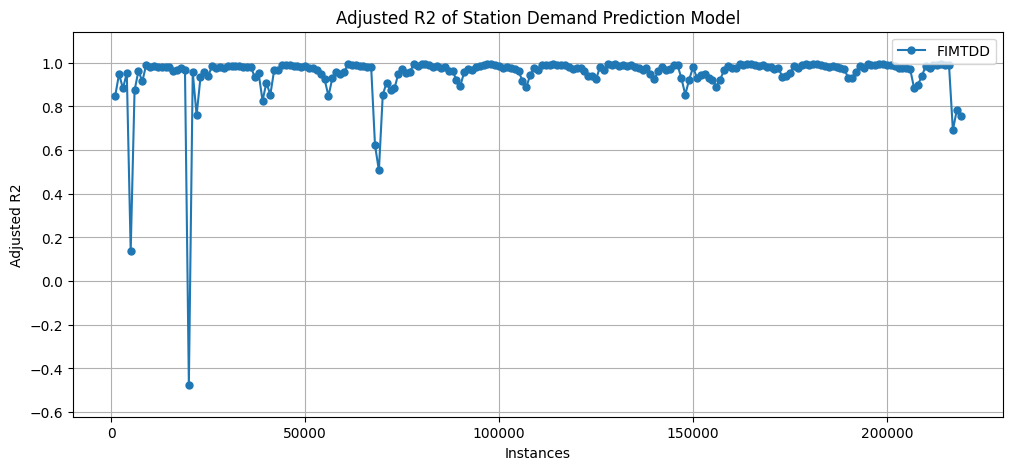
\includegraphics[scale=0.55]{r2_plot}
\end{figure}

\begin{figure}[H]
	\centering
	\caption{RMSE of Station Demand Prediction Model}
	\label{fig:rmse_plot}
	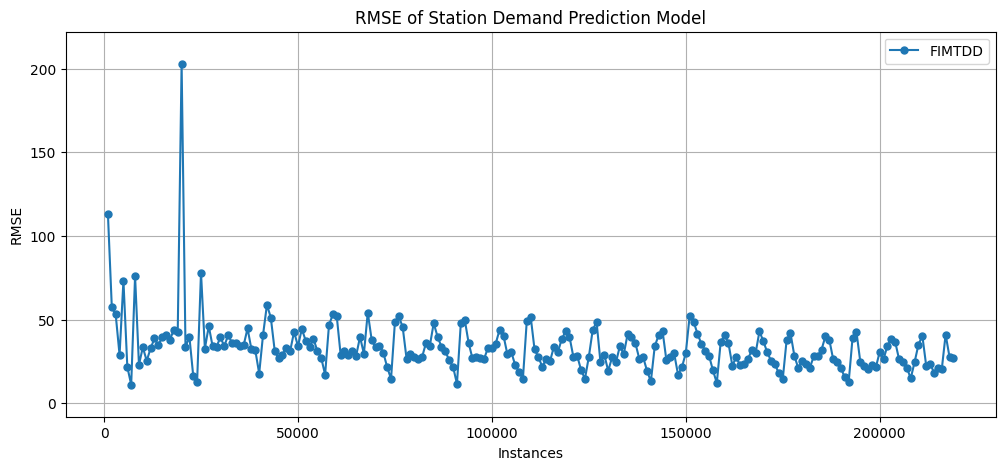
\includegraphics[scale=0.55]{rmse_plot}
\end{figure}

The Adjusted R² remains above 0.9 most of the time, even approaching 1, which demonstrates high prediction accuracy shown in Figure~\ref{fig:r2_plot}. At a few time points (such as around 10,000, 65,000, and 210,000), Adjusted R² drops sharply for a short period, with the lowest point reaching -0.5. However, the model quickly regains a high level of fit, reflecting FIMTDD's strong adaptability and robustness. Except for a few points (such as the first RMSE peak at about 210), RMSE remains in the 20–60 range for most of the time shown in Figure~\ref{fig:rmse_plot}. The overall low RMSE indicates that the prediction results have small fluctuations and controllable errors.

%\begin{figure}[H]
%	\centering
%	\caption{Predictions vs. Cround Truth of Station Demand Prediction Modell}
%	\label{fig:ground_truth}
%	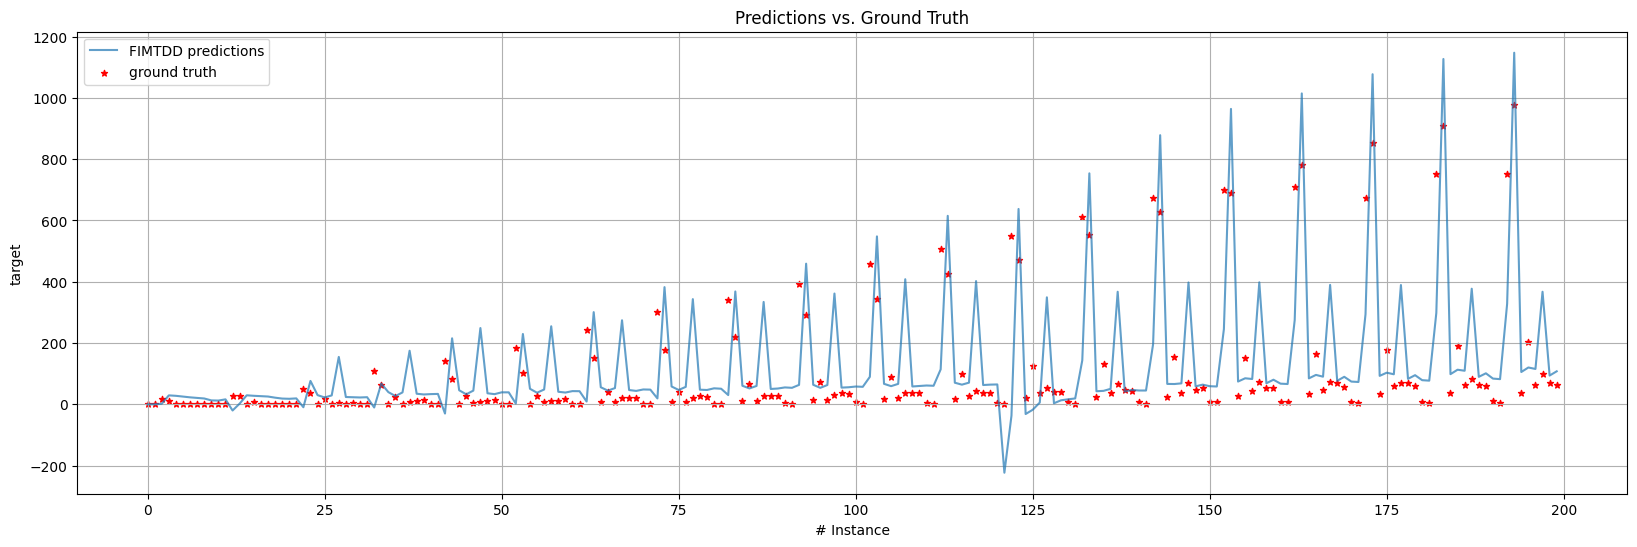
\includegraphics[scale=0.35]{ground_truth}
%\end{figure}

\subsubsection{Run real-time station recommendation system simulation}
We simulate a real-time station recommendation system. First, a random time is selected during working hours between 7:00 AM and 7:00 PM. Then, the BSD model is used to predict the busyness level of all stations.

If any busy stations are detected, the system will search for alternative stations within 1000 meters that are closer in distance and have lower predicted passenger flow.

If such less crowded stations exist, the system will recommend at least two stations to passengers.

A sample output of the simulation is shown below:

\begin{longtable}{p{4cm}p{10cm}}
	\toprule
	\textbf{Timestamp} & \textbf{Log Details} \\
	\midrule
	2024-05-29 11:50:00 & 
\begin{itemize}
	\item Detected 1 busy station: \texttt{Avenida Vale Do Tororo 327 Salvador - Bahia 40050 Brasil}
	\item Recommended alternative: \texttt{Avenida Vasco da Gama 4274 - Brotas Salvador - BA Brasil - 44784438}
	\item Distance: 843m
\end{itemize} \\
\hline

2024-05-29 11:55:00 & 
\begin{itemize}
	\item Detected 1 busy station: \texttt{Avenida Vale Do Tororo 327 Salvador - Bahia 40050 Brasil}
	\item Recommended alternative: \texttt{Avenida Vasco da Gama 4274 - Brotas Salvador - BA Brasil - 44784438}
	\item Distance: 843m
\end{itemize} \\
\hline

2024-05-29 12:00:00 & 
\begin{itemize}
	\item Detected 1 busy station: \texttt{Avenida Vale Do Tororo 327 Salvador - Bahia 40050 Brasil}
	\item Recommended alternative: \texttt{Avenida Vasco da Gama 4274 - Brotas Salvador - BA Brasil - 44784438}
	\item Distance: 843m
\end{itemize} \\
\bottomrule
\end{longtable}

\begin{table}[h]
	\centering
	\caption{Simulation Results Summary}
	\label{tab:simulation_results}
	\begin{tabular}{|c|c|c|}
		\hline
		\textbf{Timestamp} & \textbf{Busy Stations Count} & \textbf{Recommendations Count} \\ \hline
		2024-05-29 11:50 & 1 & 1 \\ \hline
		2024-05-29 11:55 & 1 & 1 \\ \hline
		2024-05-29 12:00 & 1 & 1 \\ \hline
		2024-05-29 12:05 & 1 & 1 \\ \hline
		2024-05-29 12:10 & 1 & 1 \\ \hline
		2024-05-29 12:15 & 1 & 1 \\ \hline
		2024-05-29 12:20 & 1 & 1 \\ \hline
		2024-05-29 12:25 & 1 & 1 \\ \hline
		2024-05-29 12:30 & 1 & 1 \\ \hline
		2024-05-29 12:35 & 1 & 1 \\ \hline
		2024-05-29 12:40 & 1 & 1 \\ \hline
		2024-05-29 12:45 & 1 & 1 \\ \hline
		2024-05-29 12:50 & 1 & 1 \\ \hline
		2024-05-29 12:55 & 1 & 1 \\ \hline
		2024-05-29 13:00 & 1 & 1 \\ \hline
		2024-05-29 13:05 & 1 & 1 \\ \hline
		2024-05-29 13:10 & 1 & 1 \\ \hline
		2024-05-29 13:15 & 1 & 1 \\ \hline
		2024-05-29 13:20 & 1 & 1 \\ \hline
		2024-05-29 13:25 & 1 & 1 \\ \hline
		2024-05-29 13:30 & 1 & 1 \\ \hline
		2024-05-29 13:35 & 1 & 1 \\ \hline
		2024-05-29 13:40 & 1 & 1 \\ \hline
		2024-05-29 13:45 & 1 & 1 \\ \hline
	\end{tabular}
\end{table}
\section{Discussion}
By using the BSD and SDP models to recommend alternative stations, this system aims to help solve urban traffic congestion problems. In our simulation experiments using 5-minute interval data, the results were promising — the system could effectively detect busy stations and recommend alternative stations.

However, in cases of sudden changes in passenger flow, such as during public holidays when the number of passengers increases sharply, further analysis and optimization of the system are needed to improve its response to such abnormal situations.

\section{Conclusion}

This study explores dynamic station recommendation using online learning algorithms to analyze bus station data. The proposed method takes full advantage of CapyMOA's streaming data processing capabilities, enabling real-time adaptation to changing passenger flow and avoiding the delay caused by batch learning.

According to the experimental results:

\begin{enumerate}
	\item The cumulative accuracy of the busy station detection model reached 98.330%.
	\item The cumulative adjusted R² of the station demand prediction model was 0.974.
\end{enumerate}
	
Both the BSD and SDP models achieved high overall accuracy with low fluctuation. Even when data changed suddenly, the models could quickly recover and adapt.

\section{CRediT Statement}


\bibliographystyle{apacite}  
\bibliography{references} 
	
%\section*{Appendices}

\end{document}
